\setauthor{Quirin Ecker}

Die BeamVR Applikation benötigt viele Geräte und Gegenstände um die Immersion zu gewährleisten.
Daher sind sehr viele Schritte involviert, um BeamVR in ihrer vollen Funktionalität zu genießen.
Folgende Schritte sind involviert:

\begin{itemize}
    \item Aufbau
    \item Steam VR Installation
    \item VR Headset Verbindung
    \item Tracker Verbindung
    \item Steam VR Setup
    \item Applikation Starten
    \item Beam Kalibration
    \item Full Body Tracking Kalibration
\end{itemize}


\section{Aufbau}\label{sec:aufbau}

Folgend werden alle Gegenstände und Geräte für den Aufbau in Abb.~\ref{fig:assembly} aufgelistet.

\begin{figure}
    \centering
    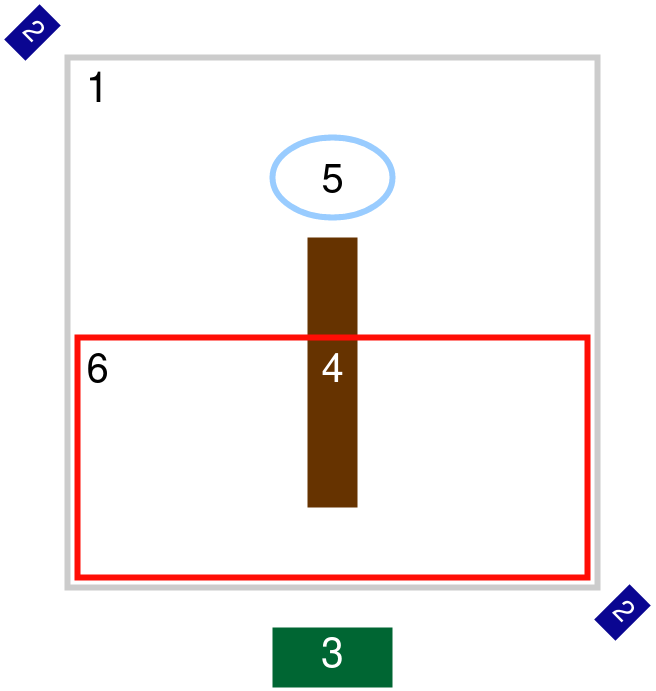
\includegraphics[scale=0.5]{pics/assemlbly}
    \caption{Aufbau}
    \label{fig:assembly}
\end{figure}

\begin{enumerate}
    \item VR Raum
    \item Lighthouses~\ref{sec:lighthouse_tracking}
    \item Monitor
    \item Balken
    \item Startposition
    \item Virtueller Abgrund
\end{enumerate}

\subsection{Erklärung}\label{subsec:description}

Die folgende Erklärung bezieht sich dabei auf die Abbildung~\ref{fig:assembly}
Der Spieler oder die Spielerin startet bei der Startposition und balanciert entlang des Balkens.
Die Base-Stations müssen diagonal zueinander positioniert werden.
Für mehr Information über die Base-Stations wird auf den Abschnitt~\ref{sec:lighthouse_tracking} verwiesen.
Der Balken sollte ca in der Mitte positioniert werden und die langen seiten sollten möglichst parallel zu den langen seiten des VR Raums sein.

Leichte Abweichungen der optimalen position sind nicht problematisch.
Größere Abweichungen können zu unerwarteten Verhalten führen.
Die echte Position des Monitors muss nicht in der gleichen Position wie in der Abbildung sein.
Dabei ist die Kennzeichnung nur für die Kalibrierung wichtig.

\section{Steam VR Installation}\label{sec:steam-vr-installation}

\begin{figure}
    \centering
    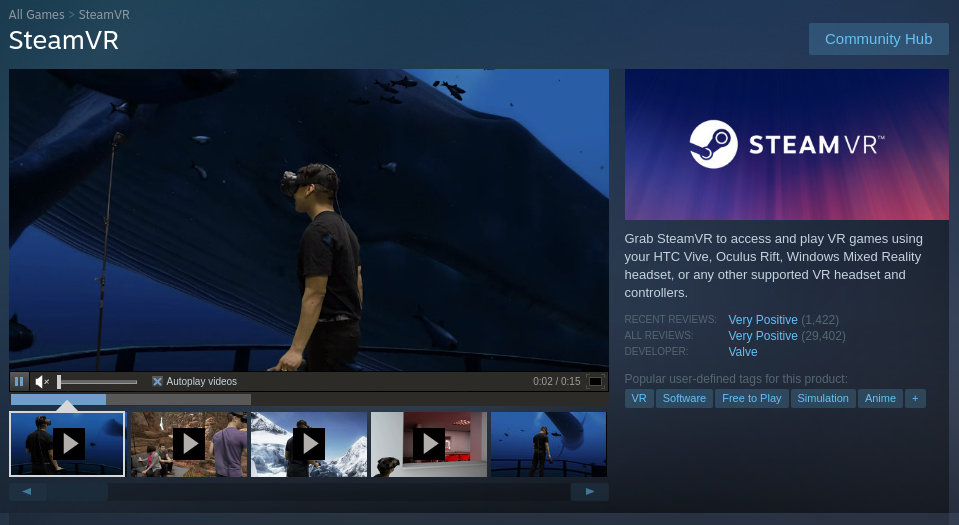
\includegraphics[scale=0.4]{pics/steam-vr-in-store}
    \caption{Steam VR Download}
    \label{fig:steam-vr-in-store}
\end{figure}

Offiziell werden die Valve Index und die HTC Brillen von BeamVR unterstützt.
Somit funktioniert die Applikation mit SteamVR.
Steam VR ist eine Software welche auf Steam herunterladbar ist.
Es ist dabei nicht wichtig, dass die SteamVR Installation vor dem Einstecken der Geräte erfolgt.
Der Download für die Software ist in dem Steam Store zu finden.
In Abb.~\ref{fig:steam-vr-in-store} ist ein Screenshot von der Steam VR Downloadseite zu sehen.

\section{VR Headset Verbindung}\label{sec:vr-headset-verbindung}

Die Verbindung von dem Headset zu dem Computer ist von Headset zu Headset unterschiedlich.
Deshalb wird in Zuge diesr Arbeit nur die Verbindung mit einer HTC Vive Pro beschrieben.
Dabei ist auch die kabellose Variante inkludiert, welche mit dem HTC Vive Wireless Adapter funktioniert.
Für mehr informationen zu dem Adapter wird auf~\ref{subsec:wireless-virtual-reality} verwiesen.

\subsection{Tethered}\label{subsec:tethered}

\begin{figure}
    \centering
    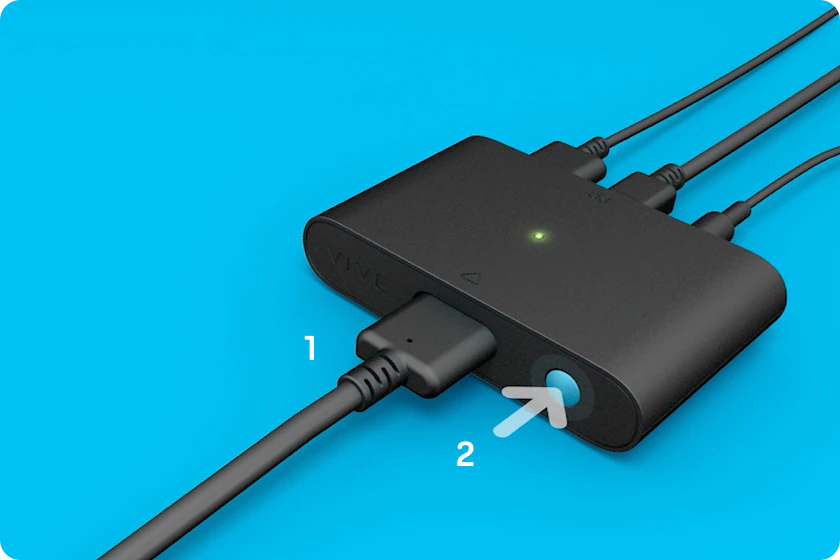
\includegraphics[scale=0.4]{pics/link-box-setup}
    \caption{Aufgesetzte Linkbox}
    \label{fig:link-box-setup}
\end{figure}


In der Box der HTC Vive Pro befindet sich eine sogenannte Linkbox.
Diese Linkbox ist die Zentralstelle, an der das Headset steckt, die Kabel zu dem Computer und das Stromkabel.
Diese Ports sind auf zwei Seiten aufgeteilt.
Eine Seite ist nur für das Headset Kabel und die andere Seite ist für den Strom und die PC-Verbindung.
Das Headset Kabel ist ein spezielles Kabel für die Brille, das Stromkabel ein Power-Adapter und die PC-Verbindung ist ein USB-A Kabel und ein Mini Displayport zu normalen Displayport Kabel~\cite{VivePro_Setup}.
In Abb.~\ref{fig:link-box-setup} ist eine aufgesetzte Linkbox zu sehen.
Für mehr Informationen wird auf~\cite{VivePro_Setup} verwiesen.

\subsection{Wireless Adapter}\label{subsec:wireless-adapter}

Mit dem Wireless Adapter kann das Headset ohne Kabel verwendet werden.
Das Aufsetzen von dem Wireless Adapter ist etwas komplizierter.
Wie bereits in dem Abschnitt~\ref{subsec:wireless-virtual-reality} braucht diese Verbindung zu dem Computer auch eine Linkbox.

\begin{figure}
    \centering
    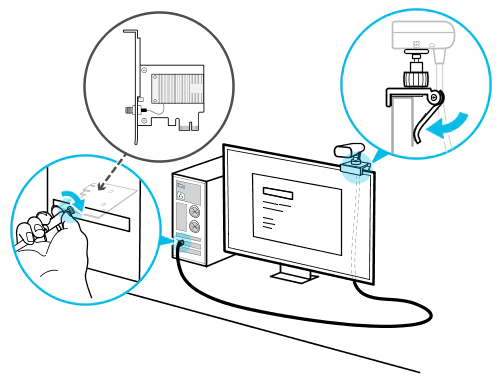
\includegraphics[scale=0.5]{pics/vive-wireless-setup-linkbox}
    \caption{Linkbox Setup~\cite{Wireless_Adapter_Setup_Docs}}
    \label{fig:vive-wireless-setup-linkbox}
\end{figure}


In diesem Fall reicht ein Kabel, welches diese Linkbox verbindet.
Dieses Kabel ist dann mit einer PCIe Karte im Computer verbunden, welche vor diesem Prozess in den Computer eingebaut werden muss.
Die Linkbox an sich muss statisch irgendwo positioniert werden.
Mögliche Orte dafür wären das der Monitor oder die Wand.
Grundsätzlich wäre es optimal, dass die Linkbox eine freie Sicht auf die VR-Brille hat~\cite{Wireless_Adapter_Setup_Docs}.
In Abb.~\ref{fig:vive-wireless-setup-linkbox} ist auf dem Monitor eine mit dem links stehenden PC verbundene Linkbox.

\begin{figure}
    \centering
    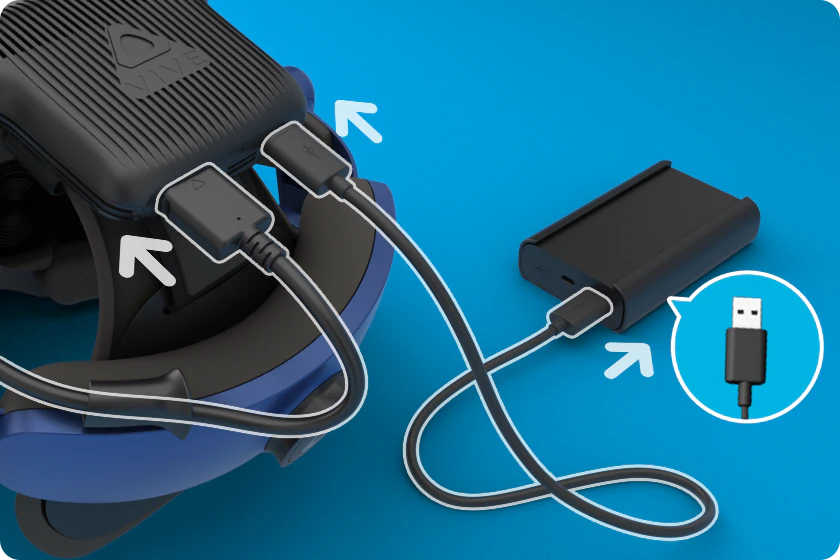
\includegraphics[scale=0.3]{pics/vive-wireless-setup-adapter}
    \caption{Angesteckter Adapter~\cite{Wireless_Adapter_Setup_Page}}
    \label{fig:vive-wireless-setup-adapter}
\end{figure}


Schlussendlich wird für das kabellose Erlebnis noch der Adapter gebraucht, welcher auf die VR-Brille angebracht wird.
Der Adapter besitzt einen Headset kabel Port und einen USB-A Port.
Inkludiert in der Box des Adapters ist ein kürzeres Headset Kabel zur verbindung des Headsets mit dem Adapter.
Der USB-Port wird für die Stromzufuhr gebraucht.
Für den Strom wird eine inkludierte Powerbank mit dem Headset verbunden mittel eines USB-A zu UBS-A Kabel~\cite{Wireless_Adapter_Setup_Page}.
In Abb.~\ref{fig:vive-wireless-setup-adapter} ist ein fertig angesteckter Adapter zu sehen.

Um den Wireless Adapter nun zu verwenden wird noch eine extra Software benötigt, die man von der HTC Vive Seite herunterladen kann.
Mit dieser sollte sich das Headset automatisch mit dem Computer über Steamvr verbinden~\cite{Wireless_Adapter_Setup_Page}.

\section{Tracker Verbindung}\label{sec:tracker-verbindung}

Genauso wie die Controller und das Headset funktionieren die Tracker mit der SteamVR Software.
Anders wie bei den Controllern ist die Verbindung zu dem Computer.
Die Verbindung wird über eine Dongle und einer Dongle Halterung gelöst.
Dabei wird die Dongle Halterung an den PC angesteckt und die Dongle in die Dongle Halterung eingesteckt~\cite{vive_tracker_setup_video_2021}.

Sobald die Tracker fertig eingesteckt sind, muss in SteamVR und bei den Trackern die Pairing Modus aktiviert werden.
In Steam VR kann dieser Modus unter \emph{SteamVR Menü > Devices > Pair Controller} gefunden werden.
Der Pairingmodus des Trackers erfolgt mit einem langen drücken des Knopfes in der Mitte des Trackers~\cite{vive_tracker_setup_video_2021}.

\section{Steam VR Setup}\label{sec:steam-vr-setup}

In der SteamVR Applikation kann unter \emph{SteamVR Menü > Room Setup} das Room Setup gefunden werden.
Das Roomsetup ist für die Kalibrierung des Raumes zuständig.
Dies beinhaltet die höhe des Bodens, die Größe des VR Raumes und die Orientierung des VR Raumes.
Bei der BeamVR Applikation ist das Setup ein wichtiger Schritt, um ein immersives Erlebnis zu erreichen.

Zum Zeitpunkt der Erstellung dieser Arbeit konnten keine zuverlässigen Informationen bezüglich des Room Setup gefunden werden.
Trotzdem zeigt sich aus Erfahrung, dass die Kalibrierung des Monitors die initiale Richtung des VR Headsets angibt.
Die Richtung des VR Headsets ist aber auch von dem Seitenverhältnis der VR Fläche abhängig.
Zeigt der Controller bei der Kalibrierung de länge des Raums entlang ist die Orientierung des Headsets trotzdem in Richtung der Breite.
Bedeutet, dass sich die Orientierung in diesem Fall gegen den Uhrzeigersinn um 90 Grad dreht.

\begin{figure}
    \centering
    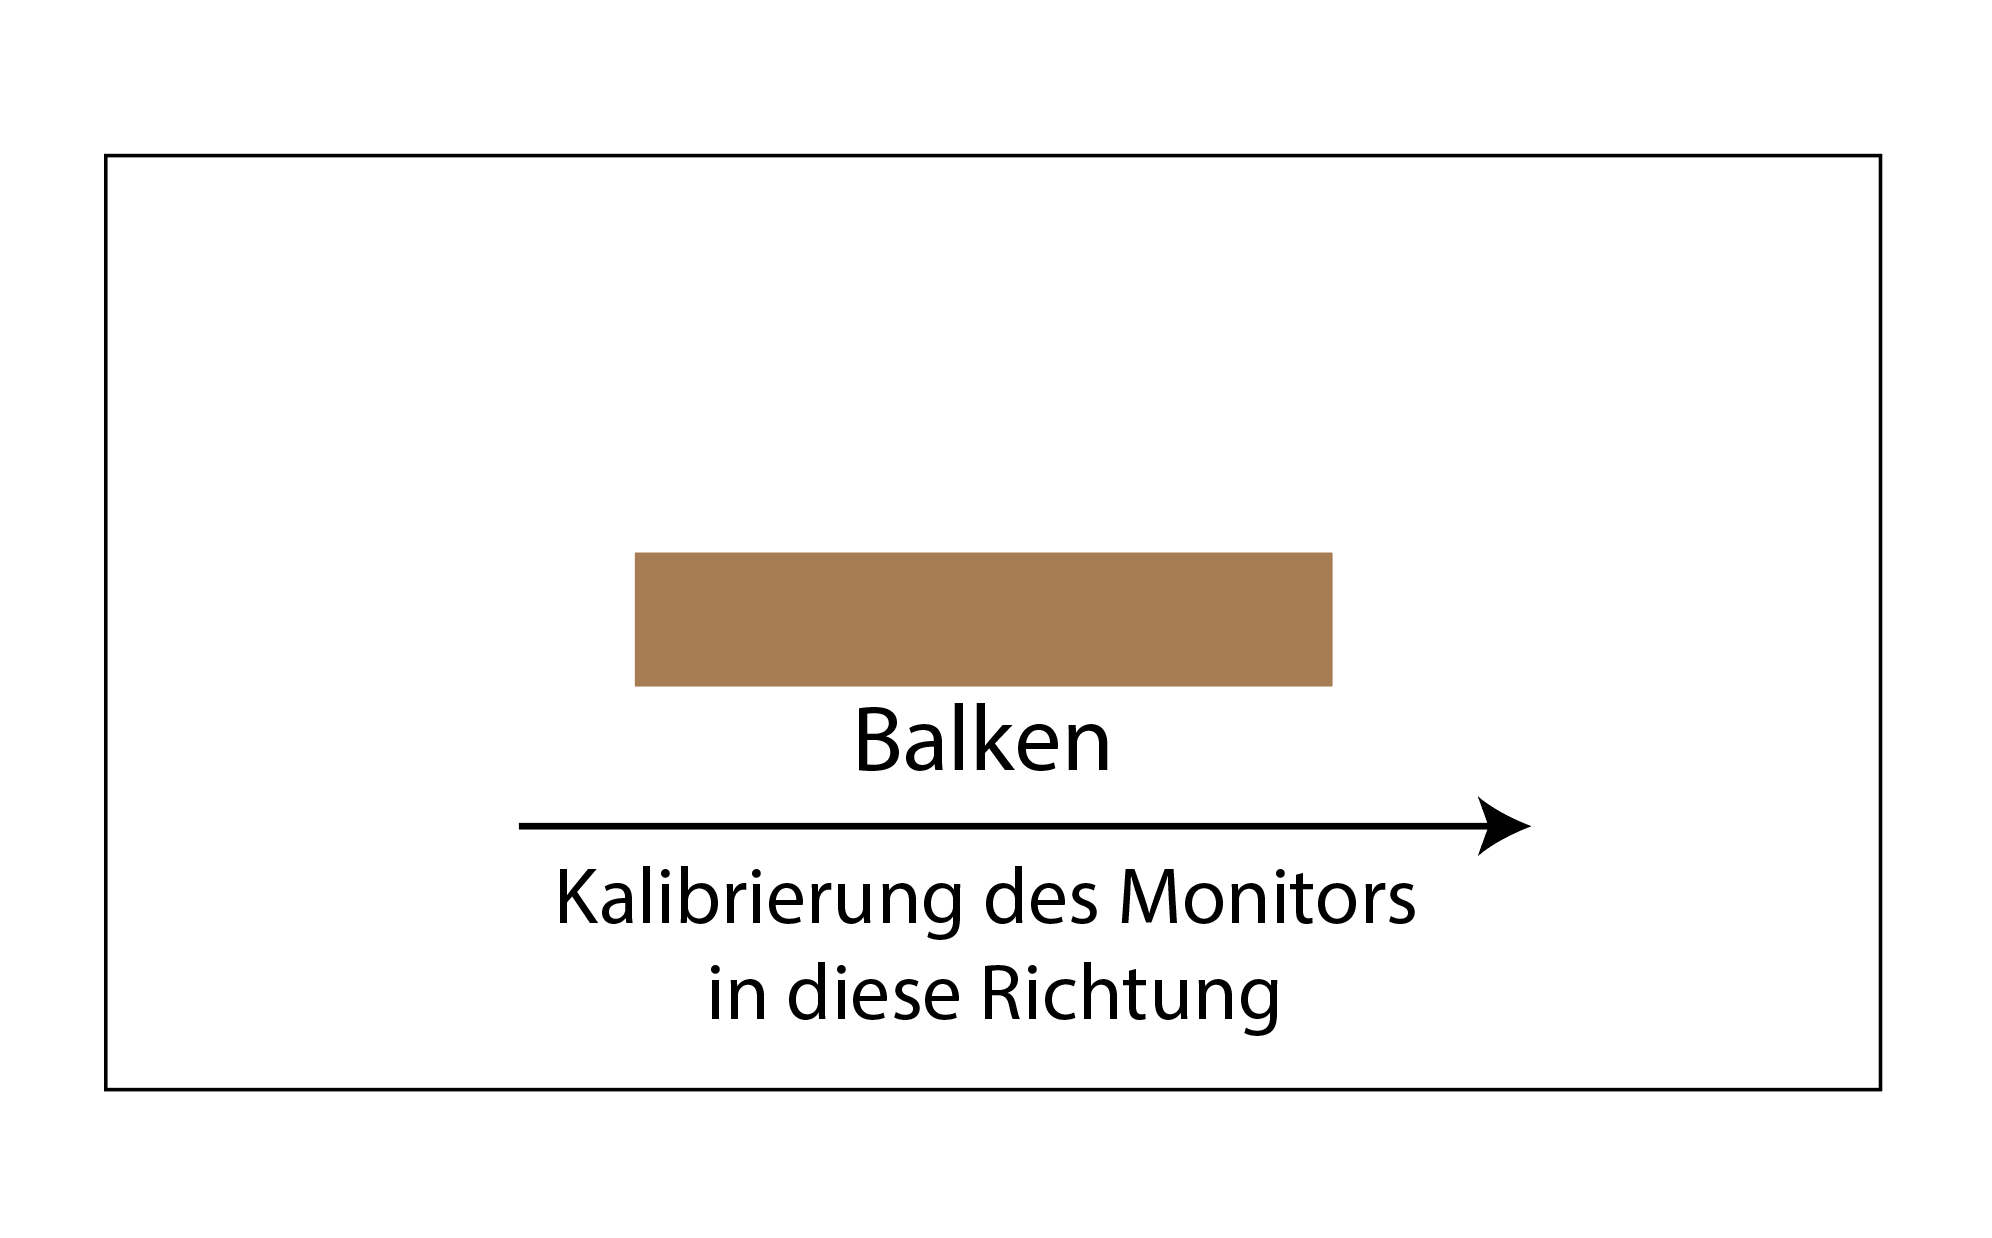
\includegraphics[scale=0.2]{pics/monitor_calibration}
    \caption{Kalibrierung des Monitors und der Maße des VR Raums}
    \label{fig:steam-vr-calibration}
\end{figure}

\begin{figure}
    \centering
    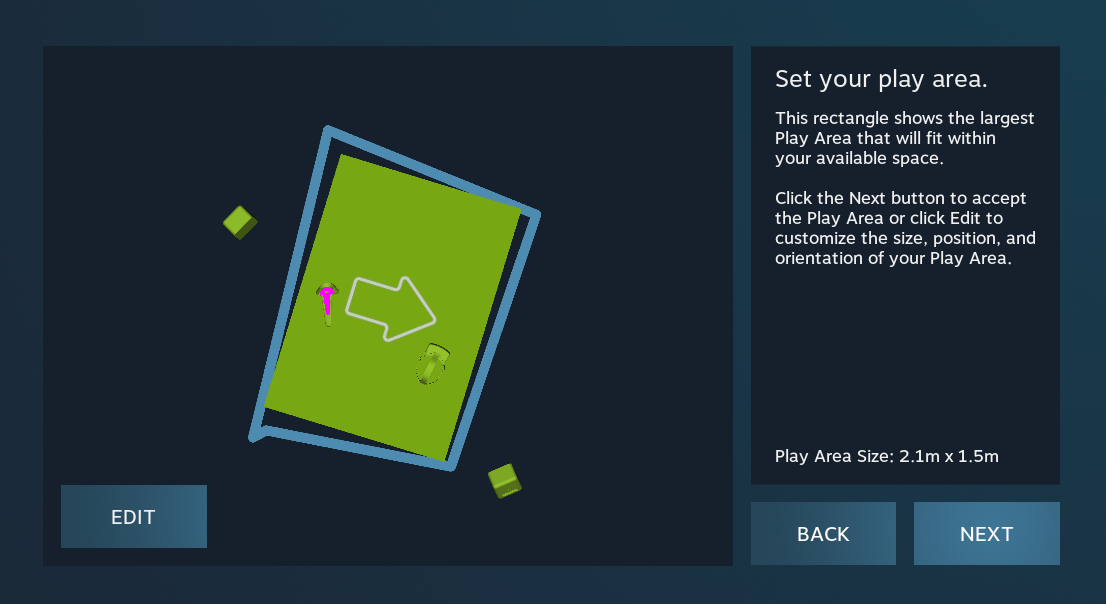
\includegraphics[scale=0.4]{pics/steam-vr-summary}
    \caption{Steam VR Setup Zusammenfassung}
    \label{fig:steam-vr-summary}
\end{figure}



Für BeamVR ist es wichtig, dass die längere Seite in die gleiche Richtung wie der Balken schaut und die kürzere seite in die andere.
Dies ist in Abb.~\ref{fig:steam-vr-calibration} abgebildet.
In der Zusammenfassung des VR Raums sollte die Orientierung wie in Abb.~\ref{fig:steam-vr-summary} ausschauen.

Bei der Kalibrierung des Bodens ist es nur wichtig, dass es möglich genau ist, damit die Gravitation wie erwarted funktioniert.
Für mehr Information über die Gravitaion wird auf~\ref{sec:gravity} verwiesen.

\section{Applikation Starten}\label{sec:run-application}

Nachdem alles aufgebaut und aufgesetzt ist kann die Applikation in Steam gestartet werden.
Die Applikation kann in dem Unity Editor gestartet werden oder als gebaute Datei.
Wichtig dabei ist, dass das Spiel bei Steam importiert wird, damit das Controller Mapping funktioniert.

\section{Beam Kalibration}\label{sec:beam-kalibration}

Bevor eine der drei Karten ausgewählt werden kann, muss noch die Beam Kalibration stattfinden.
Diese ist für die Ortung des Balkens in der digitalen Welt.
Für mehr Informationen zu der Kalibrierung wird auf den Abschnitt~\ref{sec:beam-calibration} verwiesen.
Dort wird das Setup noch genauer beschrieben.

\subsection{Full Body Tracking Kalibration}\label{subsec:full-body-tracking-calibration}

\begin{figure}
    \centering
    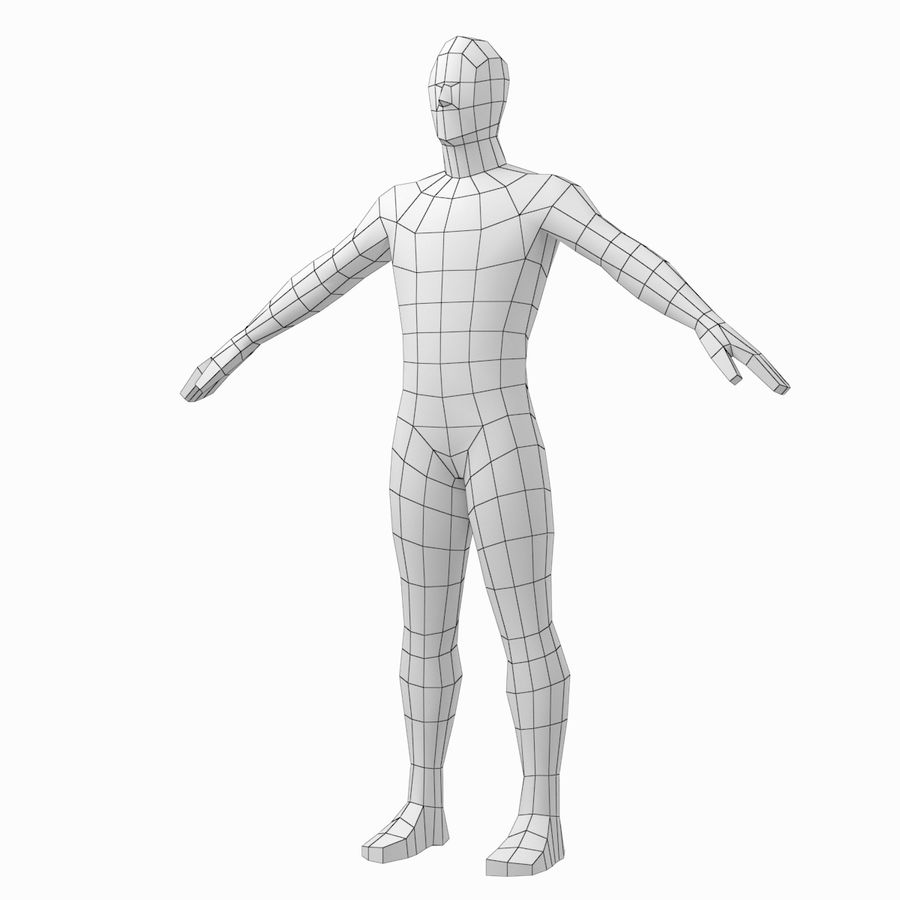
\includegraphics[scale=0.3]{pics/a-pose-human}
    \caption{A-Pose Modell~\cite{vkstudio_2020}}
    \label{fig:a-pose-human}
\end{figure}

\begin{figure}
    \centering
    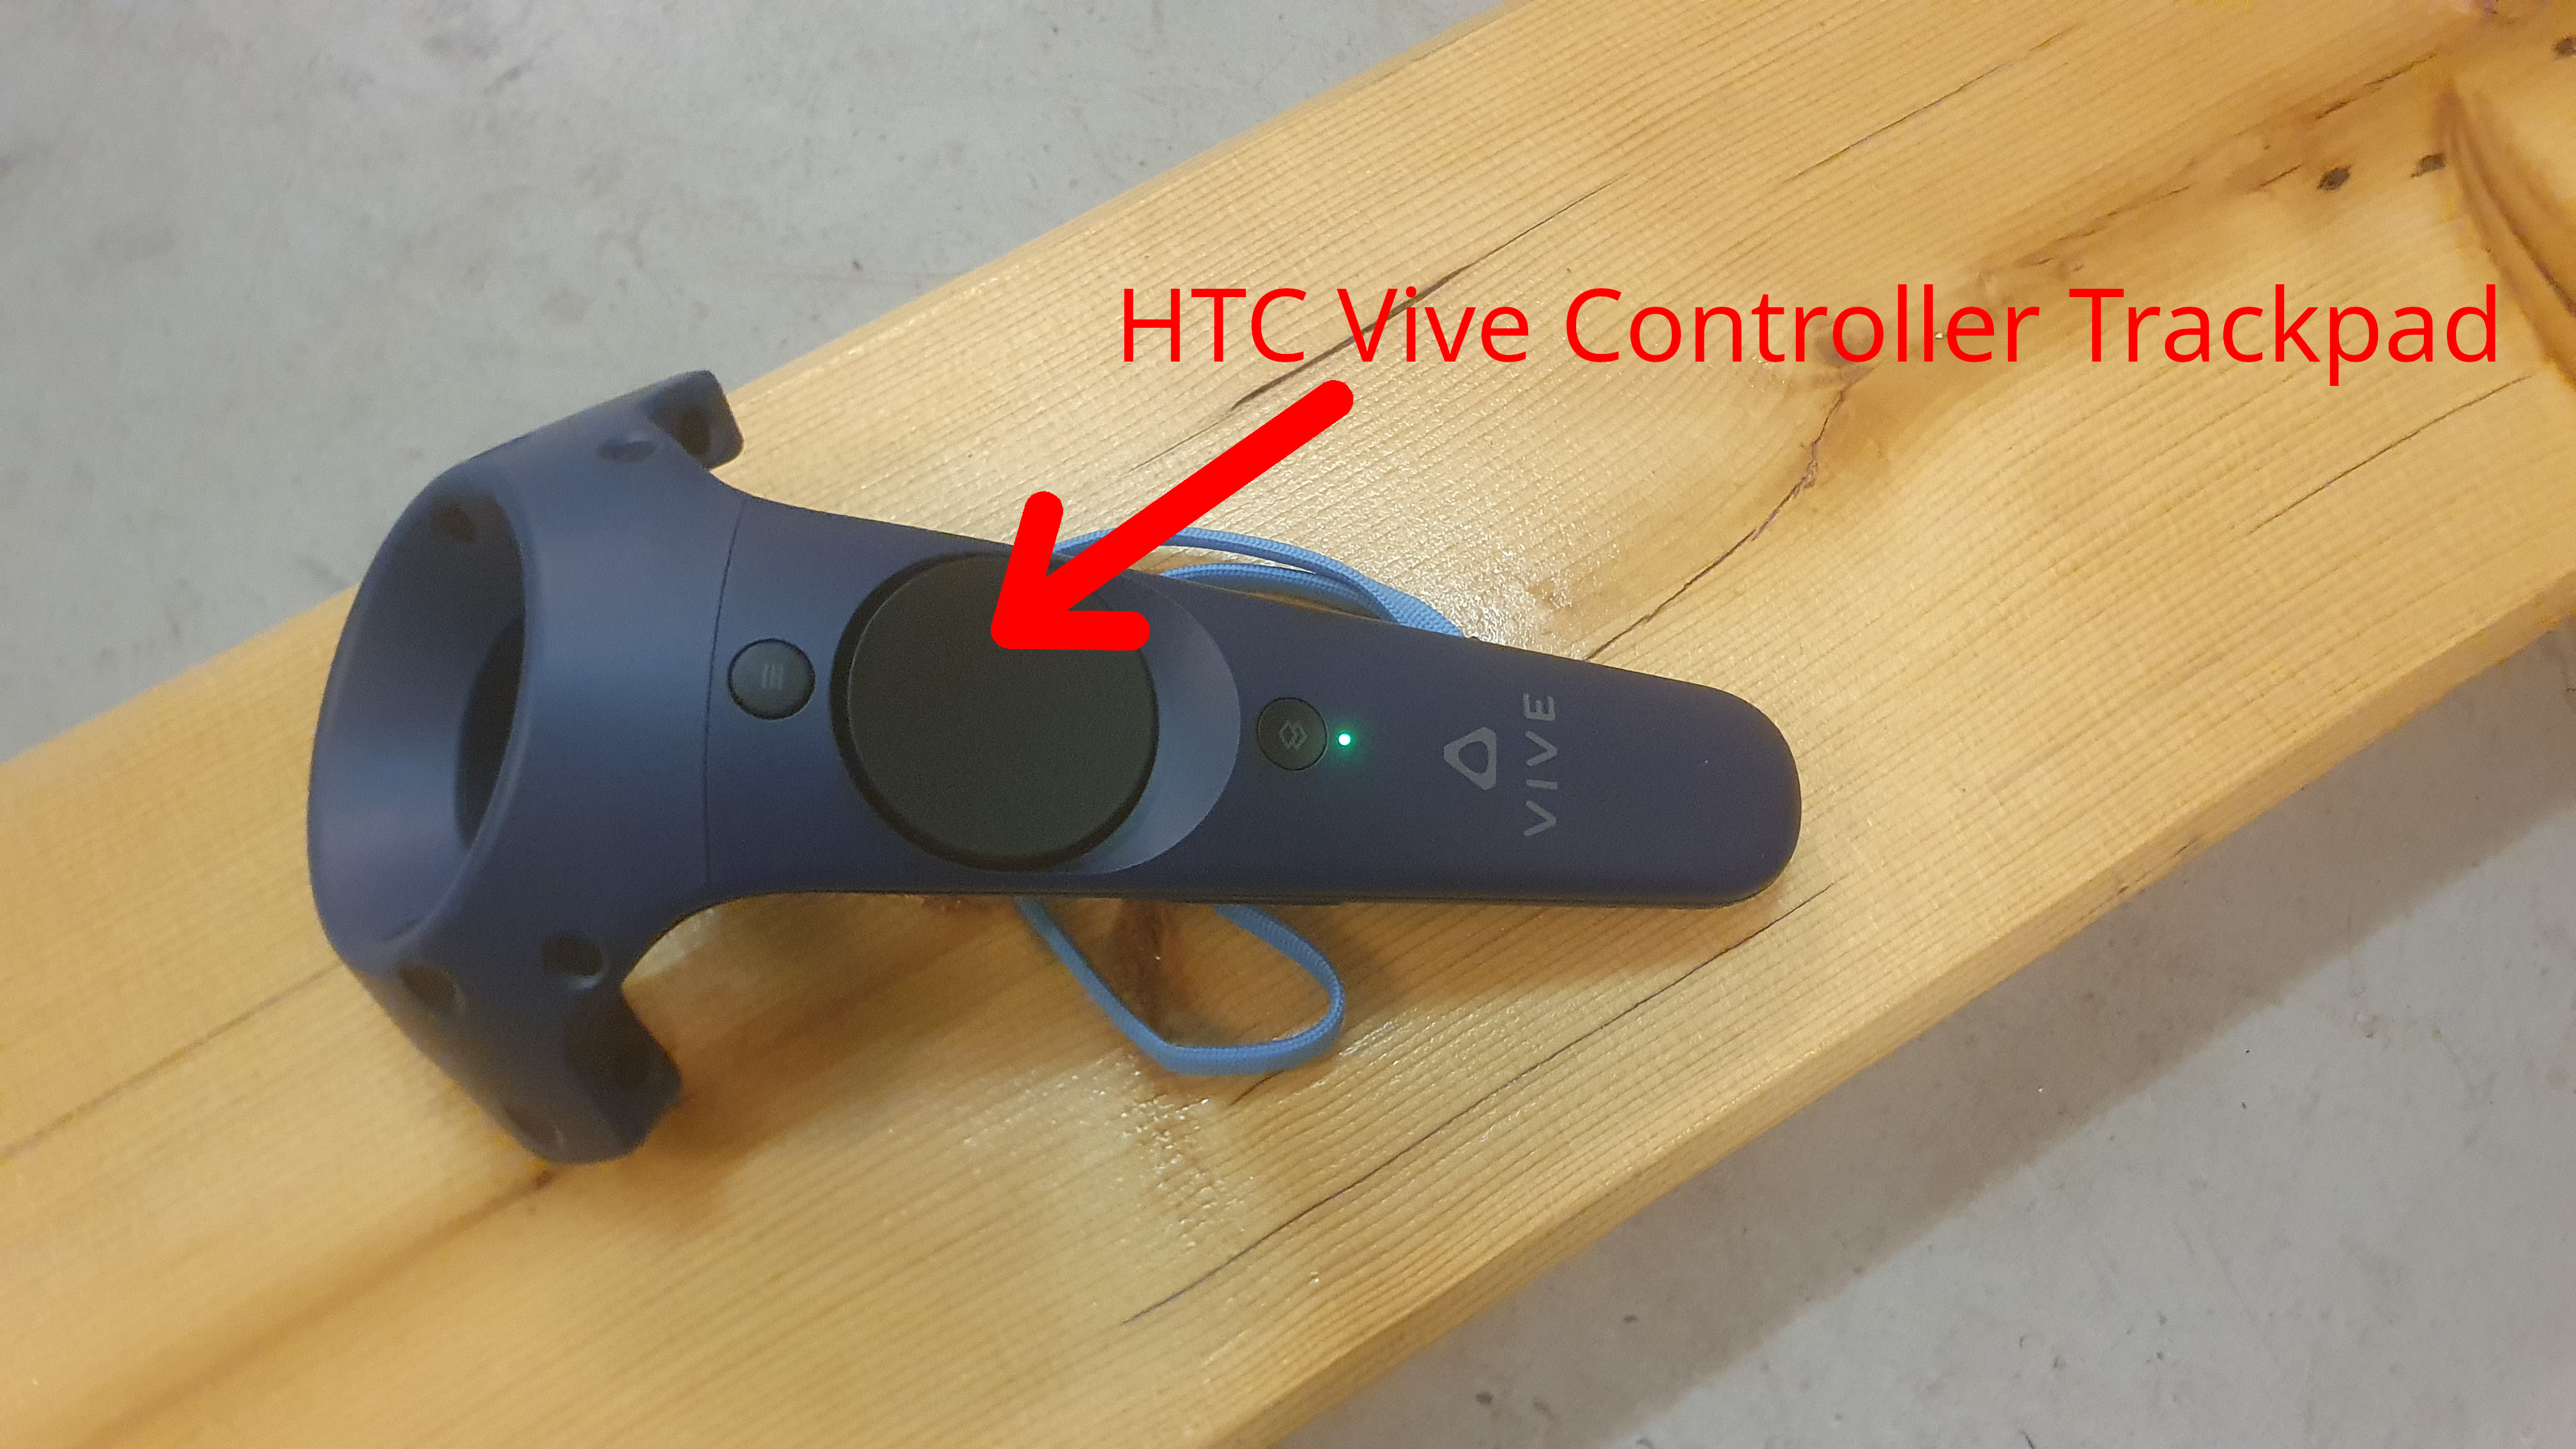
\includegraphics[scale=0.1]{pics/vive_controller_trackpad}
    \caption{Trackpad des HTC Vive Pro Controller}
    \label{fig:vive-controller-trackpad}
\end{figure}



Nach der Beam Kalibration ist es möglich eine Karte auszuwählen.
In diesen Karten steht vorne am Balken ein Spieler Modell.
Das Full Body Tracking wird durch Drücken des Trackpads auf dem Controllers aktiviert.
In Abb.~\ref{fig:vive-controller-trackpad} ist das Trackpad eines HTC Vive Controller zu sehen.

Für ein gutes Tracking sollte eine möglichst natürliche Pose, wie beispielsweise eine A-Pose, eingehalten werden.
Diese A-Pose ist in Abb.~\ref{fig:a-pose-human} abgebildet.
